\documentclass[]{article}
\usepackage{lmodern}
\usepackage{amssymb,amsmath}
\usepackage{ifxetex,ifluatex}
\usepackage{fixltx2e} % provides \textsubscript
\ifnum 0\ifxetex 1\fi\ifluatex 1\fi=0 % if pdftex
  \usepackage[T1]{fontenc}
  \usepackage[utf8]{inputenc}
\else % if luatex or xelatex
  \ifxetex
    \usepackage{mathspec}
  \else
    \usepackage{fontspec}
  \fi
  \defaultfontfeatures{Ligatures=TeX,Scale=MatchLowercase}
\fi
% use upquote if available, for straight quotes in verbatim environments
\IfFileExists{upquote.sty}{\usepackage{upquote}}{}
% use microtype if available
\IfFileExists{microtype.sty}{%
\usepackage[]{microtype}
\UseMicrotypeSet[protrusion]{basicmath} % disable protrusion for tt fonts
}{}
\PassOptionsToPackage{hyphens}{url} % url is loaded by hyperref
\usepackage[unicode=true]{hyperref}
\hypersetup{
            pdftitle={Lab4},
            pdfauthor={Justin Stott},
            pdfborder={0 0 0},
            breaklinks=true}
\urlstyle{same}  % don't use monospace font for urls
\usepackage[margin=1in]{geometry}
\usepackage{color}
\usepackage{fancyvrb}
\newcommand{\VerbBar}{|}
\newcommand{\VERB}{\Verb[commandchars=\\\{\}]}
\DefineVerbatimEnvironment{Highlighting}{Verbatim}{commandchars=\\\{\}}
% Add ',fontsize=\small' for more characters per line
\usepackage{framed}
\definecolor{shadecolor}{RGB}{248,248,248}
\newenvironment{Shaded}{\begin{snugshade}}{\end{snugshade}}
\newcommand{\KeywordTok}[1]{\textcolor[rgb]{0.13,0.29,0.53}{\textbf{#1}}}
\newcommand{\DataTypeTok}[1]{\textcolor[rgb]{0.13,0.29,0.53}{#1}}
\newcommand{\DecValTok}[1]{\textcolor[rgb]{0.00,0.00,0.81}{#1}}
\newcommand{\BaseNTok}[1]{\textcolor[rgb]{0.00,0.00,0.81}{#1}}
\newcommand{\FloatTok}[1]{\textcolor[rgb]{0.00,0.00,0.81}{#1}}
\newcommand{\ConstantTok}[1]{\textcolor[rgb]{0.00,0.00,0.00}{#1}}
\newcommand{\CharTok}[1]{\textcolor[rgb]{0.31,0.60,0.02}{#1}}
\newcommand{\SpecialCharTok}[1]{\textcolor[rgb]{0.00,0.00,0.00}{#1}}
\newcommand{\StringTok}[1]{\textcolor[rgb]{0.31,0.60,0.02}{#1}}
\newcommand{\VerbatimStringTok}[1]{\textcolor[rgb]{0.31,0.60,0.02}{#1}}
\newcommand{\SpecialStringTok}[1]{\textcolor[rgb]{0.31,0.60,0.02}{#1}}
\newcommand{\ImportTok}[1]{#1}
\newcommand{\CommentTok}[1]{\textcolor[rgb]{0.56,0.35,0.01}{\textit{#1}}}
\newcommand{\DocumentationTok}[1]{\textcolor[rgb]{0.56,0.35,0.01}{\textbf{\textit{#1}}}}
\newcommand{\AnnotationTok}[1]{\textcolor[rgb]{0.56,0.35,0.01}{\textbf{\textit{#1}}}}
\newcommand{\CommentVarTok}[1]{\textcolor[rgb]{0.56,0.35,0.01}{\textbf{\textit{#1}}}}
\newcommand{\OtherTok}[1]{\textcolor[rgb]{0.56,0.35,0.01}{#1}}
\newcommand{\FunctionTok}[1]{\textcolor[rgb]{0.00,0.00,0.00}{#1}}
\newcommand{\VariableTok}[1]{\textcolor[rgb]{0.00,0.00,0.00}{#1}}
\newcommand{\ControlFlowTok}[1]{\textcolor[rgb]{0.13,0.29,0.53}{\textbf{#1}}}
\newcommand{\OperatorTok}[1]{\textcolor[rgb]{0.81,0.36,0.00}{\textbf{#1}}}
\newcommand{\BuiltInTok}[1]{#1}
\newcommand{\ExtensionTok}[1]{#1}
\newcommand{\PreprocessorTok}[1]{\textcolor[rgb]{0.56,0.35,0.01}{\textit{#1}}}
\newcommand{\AttributeTok}[1]{\textcolor[rgb]{0.77,0.63,0.00}{#1}}
\newcommand{\RegionMarkerTok}[1]{#1}
\newcommand{\InformationTok}[1]{\textcolor[rgb]{0.56,0.35,0.01}{\textbf{\textit{#1}}}}
\newcommand{\WarningTok}[1]{\textcolor[rgb]{0.56,0.35,0.01}{\textbf{\textit{#1}}}}
\newcommand{\AlertTok}[1]{\textcolor[rgb]{0.94,0.16,0.16}{#1}}
\newcommand{\ErrorTok}[1]{\textcolor[rgb]{0.64,0.00,0.00}{\textbf{#1}}}
\newcommand{\NormalTok}[1]{#1}
\usepackage{graphicx,grffile}
\makeatletter
\def\maxwidth{\ifdim\Gin@nat@width>\linewidth\linewidth\else\Gin@nat@width\fi}
\def\maxheight{\ifdim\Gin@nat@height>\textheight\textheight\else\Gin@nat@height\fi}
\makeatother
% Scale images if necessary, so that they will not overflow the page
% margins by default, and it is still possible to overwrite the defaults
% using explicit options in \includegraphics[width, height, ...]{}
\setkeys{Gin}{width=\maxwidth,height=\maxheight,keepaspectratio}
\IfFileExists{parskip.sty}{%
\usepackage{parskip}
}{% else
\setlength{\parindent}{0pt}
\setlength{\parskip}{6pt plus 2pt minus 1pt}
}
\setlength{\emergencystretch}{3em}  % prevent overfull lines
\providecommand{\tightlist}{%
  \setlength{\itemsep}{0pt}\setlength{\parskip}{0pt}}
\setcounter{secnumdepth}{0}
% Redefines (sub)paragraphs to behave more like sections
\ifx\paragraph\undefined\else
\let\oldparagraph\paragraph
\renewcommand{\paragraph}[1]{\oldparagraph{#1}\mbox{}}
\fi
\ifx\subparagraph\undefined\else
\let\oldsubparagraph\subparagraph
\renewcommand{\subparagraph}[1]{\oldsubparagraph{#1}\mbox{}}
\fi

% set default figure placement to htbp
\makeatletter
\def\fps@figure{htbp}
\makeatother


\title{Lab4}
\author{Justin Stott}
\date{February 26, 2020}

\begin{document}
\maketitle

Examples

\begin{Shaded}
\begin{Highlighting}[]
\KeywordTok{library}\NormalTok{(ggplot2)}
\KeywordTok{library}\NormalTok{(tidyverse)}
\end{Highlighting}
\end{Shaded}

\begin{verbatim}
## -- Attaching packages ---------------------------------------------------------------------------------------------------------------------------------------------------------------- tidyverse 1.3.0 --
\end{verbatim}

\begin{verbatim}
## v tibble  2.1.3     v dplyr   0.8.4
## v tidyr   1.0.2     v stringr 1.4.0
## v readr   1.3.1     v forcats 0.5.0
## v purrr   0.3.3
\end{verbatim}

\begin{verbatim}
## -- Conflicts ------------------------------------------------------------------------------------------------------------------------------------------------------------------- tidyverse_conflicts() --
## x dplyr::filter() masks stats::filter()
## x dplyr::lag()    masks stats::lag()
\end{verbatim}

\begin{Shaded}
\begin{Highlighting}[]
\KeywordTok{library}\NormalTok{(plotly)}
\end{Highlighting}
\end{Shaded}

\begin{verbatim}
## 
## Attaching package: 'plotly'
\end{verbatim}

\begin{verbatim}
## The following object is masked from 'package:ggplot2':
## 
##     last_plot
\end{verbatim}

\begin{verbatim}
## The following object is masked from 'package:stats':
## 
##     filter
\end{verbatim}

\begin{verbatim}
## The following object is masked from 'package:graphics':
## 
##     layout
\end{verbatim}

\begin{Shaded}
\begin{Highlighting}[]
\KeywordTok{library}\NormalTok{(DT)}
\NormalTok{###############################################################################Title}

\NormalTok{bp <-}\StringTok{ }\KeywordTok{ggplot}\NormalTok{(PlantGrowth, }\KeywordTok{aes}\NormalTok{(}\DataTypeTok{x=}\NormalTok{group, }\DataTypeTok{y=}\NormalTok{weight)) }\OperatorTok{+}\StringTok{ }\KeywordTok{geom_boxplot}\NormalTok{()}
\NormalTok{bp}
\end{Highlighting}
\end{Shaded}

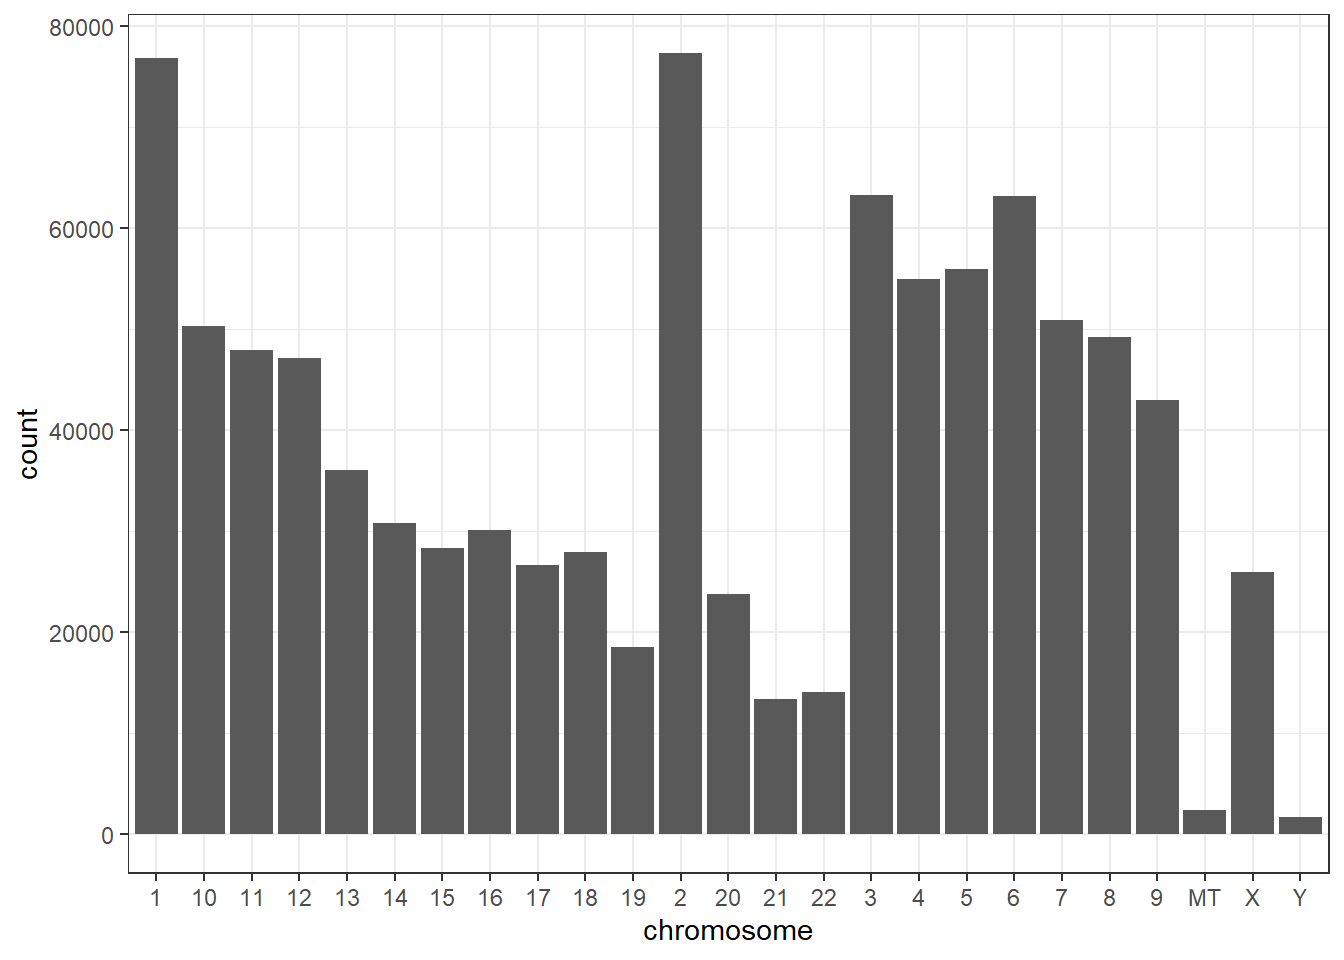
\includegraphics{Lab4_files/figure-latex/unnamed-chunk-1-1.pdf}

\begin{Shaded}
\begin{Highlighting}[]
\NormalTok{bp }\OperatorTok{+}\StringTok{ }\KeywordTok{ggtitle}\NormalTok{(}\StringTok{"Plant growth"}\NormalTok{)}
\end{Highlighting}
\end{Shaded}

\includegraphics{Lab4_files/figure-latex/unnamed-chunk-1-2.pdf}

\begin{Shaded}
\begin{Highlighting}[]
\NormalTok{## Equivalent to}
\CommentTok{# bp + labs(title="Plant growth")}

\CommentTok{# If the title is long, it can be split into multiple lines with \textbackslash{}n}
\NormalTok{bp }\OperatorTok{+}\StringTok{ }\KeywordTok{ggtitle}\NormalTok{(}\StringTok{"Plant growth with}\CharTok{\textbackslash{}n}\StringTok{different treatments"}\NormalTok{)}
\end{Highlighting}
\end{Shaded}

\includegraphics{Lab4_files/figure-latex/unnamed-chunk-1-3.pdf}

\begin{Shaded}
\begin{Highlighting}[]
\CommentTok{# Reduce line spacing and use bold text}
\NormalTok{bp }\OperatorTok{+}\StringTok{ }\KeywordTok{ggtitle}\NormalTok{(}\StringTok{"Plant growth with}\CharTok{\textbackslash{}n}\StringTok{different treatments"}\NormalTok{) }\OperatorTok{+}\StringTok{ }
\StringTok{     }\KeywordTok{theme}\NormalTok{(}\DataTypeTok{plot.title =} \KeywordTok{element_text}\NormalTok{(}\DataTypeTok{lineheight=}\NormalTok{.}\DecValTok{8}\NormalTok{, }\DataTypeTok{face=}\StringTok{"bold"}\NormalTok{))}
\end{Highlighting}
\end{Shaded}

\includegraphics{Lab4_files/figure-latex/unnamed-chunk-1-4.pdf}

\begin{Shaded}
\begin{Highlighting}[]
\NormalTok{###############################################################################Axes }
\NormalTok{bp <-}\StringTok{ }\KeywordTok{ggplot}\NormalTok{(PlantGrowth, }\KeywordTok{aes}\NormalTok{(}\DataTypeTok{x=}\NormalTok{group, }\DataTypeTok{y=}\NormalTok{weight)) }\OperatorTok{+}
\StringTok{    }\KeywordTok{geom_boxplot}\NormalTok{()}
\NormalTok{bp}
\end{Highlighting}
\end{Shaded}

\includegraphics{Lab4_files/figure-latex/unnamed-chunk-1-5.pdf}

\begin{Shaded}
\begin{Highlighting}[]
\NormalTok{bp }\OperatorTok{+}\StringTok{ }\KeywordTok{coord_flip}\NormalTok{()}
\end{Highlighting}
\end{Shaded}

\includegraphics{Lab4_files/figure-latex/unnamed-chunk-1-6.pdf}

\begin{Shaded}
\begin{Highlighting}[]
\CommentTok{# Manually set the order of a discrete-valued axis}
\NormalTok{bp }\OperatorTok{+}\StringTok{ }\KeywordTok{scale_x_discrete}\NormalTok{(}\DataTypeTok{limits=}\KeywordTok{c}\NormalTok{(}\StringTok{"trt1"}\NormalTok{,}\StringTok{"trt2"}\NormalTok{,}\StringTok{"ctrl"}\NormalTok{))}
\end{Highlighting}
\end{Shaded}

\includegraphics{Lab4_files/figure-latex/unnamed-chunk-1-7.pdf}

\begin{Shaded}
\begin{Highlighting}[]
\CommentTok{# Reverse the order of a discrete-valued axis}
\CommentTok{# Get the levels of the factor}
\NormalTok{flevels <-}\StringTok{ }\KeywordTok{levels}\NormalTok{(PlantGrowth}\OperatorTok{$}\NormalTok{group)}
\NormalTok{flevels}
\end{Highlighting}
\end{Shaded}

\begin{verbatim}
## [1] "ctrl" "trt1" "trt2"
\end{verbatim}

\begin{Shaded}
\begin{Highlighting}[]
\CommentTok{#> [1] "ctrl" "trt1" "trt2"}

\CommentTok{# Reverse the order}
\NormalTok{flevels <-}\StringTok{ }\KeywordTok{rev}\NormalTok{(flevels)}
\NormalTok{flevels}
\end{Highlighting}
\end{Shaded}

\begin{verbatim}
## [1] "trt2" "trt1" "ctrl"
\end{verbatim}

\begin{Shaded}
\begin{Highlighting}[]
\CommentTok{#> [1] "trt2" "trt1" "ctrl"}

\NormalTok{bp }\OperatorTok{+}\StringTok{ }\KeywordTok{scale_x_discrete}\NormalTok{(}\DataTypeTok{limits=}\NormalTok{flevels)}
\end{Highlighting}
\end{Shaded}

\includegraphics{Lab4_files/figure-latex/unnamed-chunk-1-8.pdf}

\begin{Shaded}
\begin{Highlighting}[]
\CommentTok{# Or it can be done in one line:}
\NormalTok{bp }\OperatorTok{+}\StringTok{ }\KeywordTok{scale_x_discrete}\NormalTok{(}\DataTypeTok{limits =} \KeywordTok{rev}\NormalTok{(}\KeywordTok{levels}\NormalTok{(PlantGrowth}\OperatorTok{$}\NormalTok{group)))}
\end{Highlighting}
\end{Shaded}

\includegraphics{Lab4_files/figure-latex/unnamed-chunk-1-9.pdf}

\begin{Shaded}
\begin{Highlighting}[]
\NormalTok{bp }\OperatorTok{+}\StringTok{ }\KeywordTok{scale_x_discrete}\NormalTok{(}\DataTypeTok{breaks=}\KeywordTok{c}\NormalTok{(}\StringTok{"ctrl"}\NormalTok{, }\StringTok{"trt1"}\NormalTok{, }\StringTok{"trt2"}\NormalTok{),}
                      \DataTypeTok{labels=}\KeywordTok{c}\NormalTok{(}\StringTok{"Control"}\NormalTok{, }\StringTok{"Treat 1"}\NormalTok{, }\StringTok{"Treat 2"}\NormalTok{))}
\end{Highlighting}
\end{Shaded}

\includegraphics{Lab4_files/figure-latex/unnamed-chunk-1-10.pdf}

\begin{Shaded}
\begin{Highlighting}[]
\CommentTok{# Hide x tick marks, labels, and grid lines}
\NormalTok{bp }\OperatorTok{+}\StringTok{ }\KeywordTok{scale_x_discrete}\NormalTok{(}\DataTypeTok{breaks=}\OtherTok{NULL}\NormalTok{)}
\end{Highlighting}
\end{Shaded}

\includegraphics{Lab4_files/figure-latex/unnamed-chunk-1-11.pdf}

\begin{Shaded}
\begin{Highlighting}[]
\CommentTok{# Hide all tick marks and labels (on X axis), but keep the gridlines}
\NormalTok{bp }\OperatorTok{+}\StringTok{ }\KeywordTok{theme}\NormalTok{(}\DataTypeTok{axis.ticks =} \KeywordTok{element_blank}\NormalTok{(), }\DataTypeTok{axis.text.x =} \KeywordTok{element_blank}\NormalTok{())}
\end{Highlighting}
\end{Shaded}

\includegraphics{Lab4_files/figure-latex/unnamed-chunk-1-12.pdf}

\begin{Shaded}
\begin{Highlighting}[]
\CommentTok{# Make sure to include 0 in the y axis}
\NormalTok{bp }\OperatorTok{+}\StringTok{ }\KeywordTok{expand_limits}\NormalTok{(}\DataTypeTok{y=}\DecValTok{0}\NormalTok{)}
\end{Highlighting}
\end{Shaded}

\includegraphics{Lab4_files/figure-latex/unnamed-chunk-1-13.pdf}

\begin{Shaded}
\begin{Highlighting}[]
\CommentTok{# Make sure to include 0 and 8 in the y axis}
\NormalTok{bp }\OperatorTok{+}\StringTok{ }\KeywordTok{expand_limits}\NormalTok{(}\DataTypeTok{y=}\KeywordTok{c}\NormalTok{(}\DecValTok{0}\NormalTok{,}\DecValTok{8}\NormalTok{))}
\end{Highlighting}
\end{Shaded}

\includegraphics{Lab4_files/figure-latex/unnamed-chunk-1-14.pdf}

\begin{Shaded}
\begin{Highlighting}[]
\CommentTok{# Set the range of a continuous-valued axis}
\CommentTok{# These are equivalent}
\NormalTok{bp }\OperatorTok{+}\StringTok{ }\KeywordTok{ylim}\NormalTok{(}\DecValTok{0}\NormalTok{, }\DecValTok{8}\NormalTok{)}
\end{Highlighting}
\end{Shaded}

\includegraphics{Lab4_files/figure-latex/unnamed-chunk-1-15.pdf}

\begin{Shaded}
\begin{Highlighting}[]
\CommentTok{# bp + scale_y_continuous(limits=c(0, 8))}

\CommentTok{# These two do the same thing; all data points outside the graphing range are}
\CommentTok{# dropped, resulting in a misleading box plot}
\NormalTok{bp }\OperatorTok{+}\StringTok{ }\KeywordTok{ylim}\NormalTok{(}\DecValTok{5}\NormalTok{, }\FloatTok{7.5}\NormalTok{)}
\end{Highlighting}
\end{Shaded}

\begin{verbatim}
## Warning: Removed 13 rows containing non-finite values (stat_boxplot).
\end{verbatim}

\includegraphics{Lab4_files/figure-latex/unnamed-chunk-1-16.pdf}

\begin{Shaded}
\begin{Highlighting}[]
\CommentTok{#> Warning: Removed 13 rows containing non-finite values (stat_boxplot).}
\CommentTok{# bp + scale_y_continuous(limits=c(5, 7.5))}

\CommentTok{# Using coord_cartesian "zooms" into the area}
\NormalTok{bp }\OperatorTok{+}\StringTok{ }\KeywordTok{coord_cartesian}\NormalTok{(}\DataTypeTok{ylim=}\KeywordTok{c}\NormalTok{(}\DecValTok{5}\NormalTok{, }\FloatTok{7.5}\NormalTok{))}
\end{Highlighting}
\end{Shaded}

\includegraphics{Lab4_files/figure-latex/unnamed-chunk-1-17.pdf}

\begin{Shaded}
\begin{Highlighting}[]
\CommentTok{# Specify tick marks directly}
\NormalTok{bp }\OperatorTok{+}\StringTok{ }\KeywordTok{coord_cartesian}\NormalTok{(}\DataTypeTok{ylim=}\KeywordTok{c}\NormalTok{(}\DecValTok{5}\NormalTok{, }\FloatTok{7.5}\NormalTok{)) }\OperatorTok{+}\StringTok{ }
\StringTok{    }\KeywordTok{scale_y_continuous}\NormalTok{(}\DataTypeTok{breaks=}\KeywordTok{seq}\NormalTok{(}\DecValTok{0}\NormalTok{, }\DecValTok{10}\NormalTok{, }\FloatTok{0.25}\NormalTok{))  }\CommentTok{# Ticks from 0-10, every .25}
\end{Highlighting}
\end{Shaded}

\includegraphics{Lab4_files/figure-latex/unnamed-chunk-1-18.pdf}

\begin{Shaded}
\begin{Highlighting}[]
\CommentTok{# Reverse order of a continuous-valued axis}
\NormalTok{bp }\OperatorTok{+}\StringTok{ }\KeywordTok{scale_y_reverse}\NormalTok{()}
\end{Highlighting}
\end{Shaded}

\includegraphics{Lab4_files/figure-latex/unnamed-chunk-1-19.pdf}

\begin{Shaded}
\begin{Highlighting}[]
\CommentTok{# Setting the tick marks on an axis}
\CommentTok{# This will show tick marks on every 0.25 from 1 to 10}
\CommentTok{# The scale will show only the ones that are within range (3.50-6.25 in this case)}
\NormalTok{bp }\OperatorTok{+}\StringTok{ }\KeywordTok{scale_y_continuous}\NormalTok{(}\DataTypeTok{breaks=}\KeywordTok{seq}\NormalTok{(}\DecValTok{1}\NormalTok{,}\DecValTok{10}\NormalTok{,}\DecValTok{1}\OperatorTok{/}\DecValTok{4}\NormalTok{))}
\end{Highlighting}
\end{Shaded}

\includegraphics{Lab4_files/figure-latex/unnamed-chunk-1-20.pdf}

\begin{Shaded}
\begin{Highlighting}[]
\CommentTok{# The breaks can be spaced unevenly}
\NormalTok{bp }\OperatorTok{+}\StringTok{ }\KeywordTok{scale_y_continuous}\NormalTok{(}\DataTypeTok{breaks=}\KeywordTok{c}\NormalTok{(}\DecValTok{4}\NormalTok{, }\FloatTok{4.25}\NormalTok{, }\FloatTok{4.5}\NormalTok{, }\DecValTok{5}\NormalTok{, }\DecValTok{6}\NormalTok{,}\DecValTok{8}\NormalTok{))}
\end{Highlighting}
\end{Shaded}

\includegraphics{Lab4_files/figure-latex/unnamed-chunk-1-21.pdf}

\begin{Shaded}
\begin{Highlighting}[]
\CommentTok{# Suppress ticks and gridlines}
\NormalTok{bp }\OperatorTok{+}\StringTok{ }\KeywordTok{scale_y_continuous}\NormalTok{(}\DataTypeTok{breaks=}\OtherTok{NULL}\NormalTok{)}
\end{Highlighting}
\end{Shaded}

\includegraphics{Lab4_files/figure-latex/unnamed-chunk-1-22.pdf}

\begin{Shaded}
\begin{Highlighting}[]
\CommentTok{# Hide tick marks and labels (on Y axis), but keep the gridlines}
\NormalTok{bp }\OperatorTok{+}\StringTok{ }\KeywordTok{theme}\NormalTok{(}\DataTypeTok{axis.ticks =} \KeywordTok{element_blank}\NormalTok{(), }\DataTypeTok{axis.text.y =} \KeywordTok{element_blank}\NormalTok{())}
\end{Highlighting}
\end{Shaded}

\includegraphics{Lab4_files/figure-latex/unnamed-chunk-1-23.pdf}

\begin{Shaded}
\begin{Highlighting}[]
\CommentTok{# Create some noisy exponentially-distributed data}
\KeywordTok{set.seed}\NormalTok{(}\DecValTok{201}\NormalTok{)}
\NormalTok{n <-}\StringTok{ }\DecValTok{100}
\NormalTok{dat <-}\StringTok{ }\KeywordTok{data.frame}\NormalTok{(}
    \DataTypeTok{xval =}\NormalTok{ (}\DecValTok{1}\OperatorTok{:}\NormalTok{n}\OperatorTok{+}\KeywordTok{rnorm}\NormalTok{(n,}\DataTypeTok{sd=}\DecValTok{5}\NormalTok{))}\OperatorTok{/}\DecValTok{20}\NormalTok{,}
    \DataTypeTok{yval =} \DecValTok{2}\OperatorTok{*}\DecValTok{2}\OperatorTok{^}\NormalTok{((}\DecValTok{1}\OperatorTok{:}\NormalTok{n}\OperatorTok{+}\KeywordTok{rnorm}\NormalTok{(n,}\DataTypeTok{sd=}\DecValTok{5}\NormalTok{))}\OperatorTok{/}\DecValTok{20}\NormalTok{)}
\NormalTok{)}

\CommentTok{# A scatterplot with regular (linear) axis scaling}
\NormalTok{sp <-}\StringTok{ }\KeywordTok{ggplot}\NormalTok{(dat, }\KeywordTok{aes}\NormalTok{(xval, yval)) }\OperatorTok{+}\StringTok{ }\KeywordTok{geom_point}\NormalTok{()}
\NormalTok{sp}
\end{Highlighting}
\end{Shaded}

\includegraphics{Lab4_files/figure-latex/unnamed-chunk-1-24.pdf}

\begin{Shaded}
\begin{Highlighting}[]
\CommentTok{# log2 scaling of the y axis (with visually-equal spacing)}
\KeywordTok{library}\NormalTok{(scales)     }\CommentTok{# Need the scales package}
\end{Highlighting}
\end{Shaded}

\begin{verbatim}
## 
## Attaching package: 'scales'
\end{verbatim}

\begin{verbatim}
## The following object is masked from 'package:purrr':
## 
##     discard
\end{verbatim}

\begin{verbatim}
## The following object is masked from 'package:readr':
## 
##     col_factor
\end{verbatim}

\begin{Shaded}
\begin{Highlighting}[]
\NormalTok{sp }\OperatorTok{+}\StringTok{ }\KeywordTok{scale_y_continuous}\NormalTok{(}\DataTypeTok{trans=}\KeywordTok{log2_trans}\NormalTok{())}
\end{Highlighting}
\end{Shaded}

\includegraphics{Lab4_files/figure-latex/unnamed-chunk-1-25.pdf}

\begin{Shaded}
\begin{Highlighting}[]
\CommentTok{# log2 coordinate transformation (with visually-diminishing spacing)}
\NormalTok{sp }\OperatorTok{+}\StringTok{ }\KeywordTok{coord_trans}\NormalTok{(}\DataTypeTok{y=}\StringTok{"log2"}\NormalTok{)}
\end{Highlighting}
\end{Shaded}

\includegraphics{Lab4_files/figure-latex/unnamed-chunk-1-26.pdf}

\begin{Shaded}
\begin{Highlighting}[]
\NormalTok{sp }\OperatorTok{+}\StringTok{ }\KeywordTok{scale_y_continuous}\NormalTok{(}\DataTypeTok{trans =} \KeywordTok{log2_trans}\NormalTok{(),}
                        \DataTypeTok{breaks =} \KeywordTok{trans_breaks}\NormalTok{(}\StringTok{"log2"}\NormalTok{, }\ControlFlowTok{function}\NormalTok{(x) }\DecValTok{2}\OperatorTok{^}\NormalTok{x),}
                        \DataTypeTok{labels =} \KeywordTok{trans_format}\NormalTok{(}\StringTok{"log2"}\NormalTok{, }\KeywordTok{math_format}\NormalTok{(}\DecValTok{2}\OperatorTok{^}\NormalTok{.x)))}
\end{Highlighting}
\end{Shaded}

\includegraphics{Lab4_files/figure-latex/unnamed-chunk-1-27.pdf}

\begin{Shaded}
\begin{Highlighting}[]
\KeywordTok{set.seed}\NormalTok{(}\DecValTok{205}\NormalTok{)}
\NormalTok{n <-}\StringTok{ }\DecValTok{100}
\NormalTok{dat10 <-}\StringTok{ }\KeywordTok{data.frame}\NormalTok{(}
    \DataTypeTok{xval =}\NormalTok{ (}\DecValTok{1}\OperatorTok{:}\NormalTok{n}\OperatorTok{+}\KeywordTok{rnorm}\NormalTok{(n,}\DataTypeTok{sd=}\DecValTok{5}\NormalTok{))}\OperatorTok{/}\DecValTok{20}\NormalTok{,}
    \DataTypeTok{yval =} \DecValTok{10}\OperatorTok{*}\DecValTok{10}\OperatorTok{^}\NormalTok{((}\DecValTok{1}\OperatorTok{:}\NormalTok{n}\OperatorTok{+}\KeywordTok{rnorm}\NormalTok{(n,}\DataTypeTok{sd=}\DecValTok{5}\NormalTok{))}\OperatorTok{/}\DecValTok{20}\NormalTok{)}
\NormalTok{)}

\NormalTok{sp10 <-}\StringTok{ }\KeywordTok{ggplot}\NormalTok{(dat10, }\KeywordTok{aes}\NormalTok{(xval, yval)) }\OperatorTok{+}\StringTok{ }\KeywordTok{geom_point}\NormalTok{()}

\CommentTok{# log10}
\NormalTok{sp10 }\OperatorTok{+}\StringTok{ }\KeywordTok{scale_y_log10}\NormalTok{()}
\end{Highlighting}
\end{Shaded}

\includegraphics{Lab4_files/figure-latex/unnamed-chunk-1-28.pdf}

\begin{Shaded}
\begin{Highlighting}[]
\CommentTok{# log10 with exponents on tick labels}
\NormalTok{sp10 }\OperatorTok{+}\StringTok{ }\KeywordTok{scale_y_log10}\NormalTok{(}\DataTypeTok{breaks =} \KeywordTok{trans_breaks}\NormalTok{(}\StringTok{"log10"}\NormalTok{, }\ControlFlowTok{function}\NormalTok{(x) }\DecValTok{10}\OperatorTok{^}\NormalTok{x),}
                     \DataTypeTok{labels =} \KeywordTok{trans_format}\NormalTok{(}\StringTok{"log10"}\NormalTok{, }\KeywordTok{math_format}\NormalTok{(}\DecValTok{10}\OperatorTok{^}\NormalTok{.x)))}
\end{Highlighting}
\end{Shaded}

\includegraphics{Lab4_files/figure-latex/unnamed-chunk-1-29.pdf}

\begin{Shaded}
\begin{Highlighting}[]
\CommentTok{# Data where x ranges from 0-10, y ranges from 0-30}
\KeywordTok{set.seed}\NormalTok{(}\DecValTok{202}\NormalTok{)}
\NormalTok{dat <-}\StringTok{ }\KeywordTok{data.frame}\NormalTok{(}
    \DataTypeTok{xval =} \KeywordTok{runif}\NormalTok{(}\DecValTok{40}\NormalTok{,}\DecValTok{0}\NormalTok{,}\DecValTok{10}\NormalTok{),}
    \DataTypeTok{yval =} \KeywordTok{runif}\NormalTok{(}\DecValTok{40}\NormalTok{,}\DecValTok{0}\NormalTok{,}\DecValTok{30}\NormalTok{)}
\NormalTok{)}
\NormalTok{sp <-}\StringTok{ }\KeywordTok{ggplot}\NormalTok{(dat, }\KeywordTok{aes}\NormalTok{(xval, yval)) }\OperatorTok{+}\StringTok{ }\KeywordTok{geom_point}\NormalTok{()}

\CommentTok{# Force equal scaling}
\NormalTok{sp }\OperatorTok{+}\StringTok{ }\KeywordTok{coord_fixed}\NormalTok{()}
\end{Highlighting}
\end{Shaded}

\includegraphics{Lab4_files/figure-latex/unnamed-chunk-1-30.pdf}

\begin{Shaded}
\begin{Highlighting}[]
\CommentTok{# Equal scaling, with each 1 on the x axis the same length as y on x axis}
\NormalTok{sp }\OperatorTok{+}\StringTok{ }\KeywordTok{coord_fixed}\NormalTok{(}\DataTypeTok{ratio=}\DecValTok{1}\OperatorTok{/}\DecValTok{3}\NormalTok{)}
\end{Highlighting}
\end{Shaded}

\includegraphics{Lab4_files/figure-latex/unnamed-chunk-1-31.pdf}

\begin{Shaded}
\begin{Highlighting}[]
\NormalTok{bp }\OperatorTok{+}\StringTok{ }\KeywordTok{theme}\NormalTok{(}\DataTypeTok{axis.title.x =} \KeywordTok{element_blank}\NormalTok{()) }\OperatorTok{+}\StringTok{   }\CommentTok{# Remove x-axis label}
\StringTok{     }\KeywordTok{ylab}\NormalTok{(}\StringTok{"Weight (Kg)"}\NormalTok{)                       }\CommentTok{# Set y-axis label}
\end{Highlighting}
\end{Shaded}

\includegraphics{Lab4_files/figure-latex/unnamed-chunk-1-32.pdf}

\begin{Shaded}
\begin{Highlighting}[]
\CommentTok{# Also possible to set the axis label with the scale}
\CommentTok{# Note that vertical space is still reserved for x's label}
\NormalTok{bp }\OperatorTok{+}\StringTok{ }\KeywordTok{scale_x_discrete}\NormalTok{(}\DataTypeTok{name=}\StringTok{""}\NormalTok{) }\OperatorTok{+}
\StringTok{     }\KeywordTok{scale_y_continuous}\NormalTok{(}\DataTypeTok{name=}\StringTok{"Weight (Kg)"}\NormalTok{)}
\end{Highlighting}
\end{Shaded}

\includegraphics{Lab4_files/figure-latex/unnamed-chunk-1-33.pdf}

\begin{Shaded}
\begin{Highlighting}[]
\CommentTok{# Change font options:}
\CommentTok{# X-axis label: bold, red, and 20 points}
\CommentTok{# X-axis tick marks: rotate 90 degrees CCW, move to the left a bit (using vjust,}
\CommentTok{#   since the labels are rotated), and 16 points}
\NormalTok{bp }\OperatorTok{+}\StringTok{ }\KeywordTok{theme}\NormalTok{(}\DataTypeTok{axis.title.x =} \KeywordTok{element_text}\NormalTok{(}\DataTypeTok{face=}\StringTok{"bold"}\NormalTok{, }\DataTypeTok{colour=}\StringTok{"#990000"}\NormalTok{, }\DataTypeTok{size=}\DecValTok{20}\NormalTok{),}
           \DataTypeTok{axis.text.x  =} \KeywordTok{element_text}\NormalTok{(}\DataTypeTok{angle=}\DecValTok{90}\NormalTok{, }\DataTypeTok{vjust=}\FloatTok{0.5}\NormalTok{, }\DataTypeTok{size=}\DecValTok{16}\NormalTok{))}
\end{Highlighting}
\end{Shaded}

\includegraphics{Lab4_files/figure-latex/unnamed-chunk-1-34.pdf}

\begin{Shaded}
\begin{Highlighting}[]
\CommentTok{# Label formatters}
\KeywordTok{library}\NormalTok{(scales)   }\CommentTok{# Need the scales package}
\NormalTok{bp }\OperatorTok{+}\StringTok{ }\KeywordTok{scale_y_continuous}\NormalTok{(}\DataTypeTok{labels=}\NormalTok{percent) }\OperatorTok{+}
\StringTok{     }\KeywordTok{scale_x_discrete}\NormalTok{(}\DataTypeTok{labels=}\NormalTok{abbreviate)  }\CommentTok{# In this particular case, it has no effect}
\end{Highlighting}
\end{Shaded}

\includegraphics{Lab4_files/figure-latex/unnamed-chunk-1-35.pdf}

\begin{Shaded}
\begin{Highlighting}[]
\CommentTok{# Self-defined formatting function for times.}
\NormalTok{timeHMS_formatter <-}\StringTok{ }\ControlFlowTok{function}\NormalTok{(x) \{}
\NormalTok{    h <-}\StringTok{ }\KeywordTok{floor}\NormalTok{(x}\OperatorTok{/}\DecValTok{60}\NormalTok{)}
\NormalTok{    m <-}\StringTok{ }\KeywordTok{floor}\NormalTok{(x }\OperatorTok\StringTok{ }\DecValTok{60}\NormalTok{)}
\NormalTok{    s <-}\StringTok{ }\KeywordTok{round}\NormalTok{(}\DecValTok{60}\OperatorTok{*}\NormalTok{(x }\OperatorTok\StringTok{ }\DecValTok{1}\NormalTok{))                   }\CommentTok{# Round to nearest second}
\NormalTok{    lab <-}\StringTok{ }\KeywordTok{sprintf}\NormalTok{(}\StringTok{'%02d:%02d:%02d'}\NormalTok{, h, m, s) }\CommentTok{# Format the strings as HH:MM:SS}
\NormalTok{    lab <-}\StringTok{ }\KeywordTok{gsub}\NormalTok{(}\StringTok{'^00:'}\NormalTok{, }\StringTok{''}\NormalTok{, lab)              }\CommentTok{# Remove leading 00: if present}
\NormalTok{    lab <-}\StringTok{ }\KeywordTok{gsub}\NormalTok{(}\StringTok{'^0'}\NormalTok{, }\StringTok{''}\NormalTok{, lab)                }\CommentTok{# Remove leading 0 if present}
\NormalTok{\}}

\NormalTok{bp }\OperatorTok{+}\StringTok{ }\KeywordTok{scale_y_continuous}\NormalTok{(}\DataTypeTok{label=}\NormalTok{timeHMS_formatter)}
\end{Highlighting}
\end{Shaded}

\includegraphics{Lab4_files/figure-latex/unnamed-chunk-1-36.pdf}

\begin{Shaded}
\begin{Highlighting}[]
\CommentTok{# Hide all the gridlines}
\NormalTok{bp }\OperatorTok{+}\StringTok{ }\KeywordTok{theme}\NormalTok{(}\DataTypeTok{panel.grid.minor=}\KeywordTok{element_blank}\NormalTok{(),}
           \DataTypeTok{panel.grid.major=}\KeywordTok{element_blank}\NormalTok{())}
\end{Highlighting}
\end{Shaded}

\includegraphics{Lab4_files/figure-latex/unnamed-chunk-1-37.pdf}

\begin{Shaded}
\begin{Highlighting}[]
\CommentTok{# Hide just the minor gridlines}
\NormalTok{bp }\OperatorTok{+}\StringTok{ }\KeywordTok{theme}\NormalTok{(}\DataTypeTok{panel.grid.minor=}\KeywordTok{element_blank}\NormalTok{())}
\end{Highlighting}
\end{Shaded}

\includegraphics{Lab4_files/figure-latex/unnamed-chunk-1-38.pdf}

\begin{Shaded}
\begin{Highlighting}[]
\CommentTok{# Hide all the vertical gridlines}
\NormalTok{bp }\OperatorTok{+}\StringTok{ }\KeywordTok{theme}\NormalTok{(}\DataTypeTok{panel.grid.minor.x=}\KeywordTok{element_blank}\NormalTok{(),}
           \DataTypeTok{panel.grid.major.x=}\KeywordTok{element_blank}\NormalTok{())}
\end{Highlighting}
\end{Shaded}

\includegraphics{Lab4_files/figure-latex/unnamed-chunk-1-39.pdf}

\begin{Shaded}
\begin{Highlighting}[]
\CommentTok{# Hide all the horizontal gridlines}
\NormalTok{bp }\OperatorTok{+}\StringTok{ }\KeywordTok{theme}\NormalTok{(}\DataTypeTok{panel.grid.minor.y=}\KeywordTok{element_blank}\NormalTok{(),}
           \DataTypeTok{panel.grid.major.y=}\KeywordTok{element_blank}\NormalTok{())}
\end{Highlighting}
\end{Shaded}

\includegraphics{Lab4_files/figure-latex/unnamed-chunk-1-40.pdf}

\begin{Shaded}
\begin{Highlighting}[]
\NormalTok{###############################################################################Legend}

\CommentTok{# Remove legend for a particular aesthetic (fill)}
\NormalTok{bp }\OperatorTok{+}\StringTok{ }\KeywordTok{guides}\NormalTok{(}\DataTypeTok{fill=}\OtherTok{FALSE}\NormalTok{)}
\end{Highlighting}
\end{Shaded}

\includegraphics{Lab4_files/figure-latex/unnamed-chunk-1-41.pdf}

\begin{Shaded}
\begin{Highlighting}[]
\CommentTok{# It can also be done when specifying the scale}
\NormalTok{bp }\OperatorTok{+}\StringTok{ }\KeywordTok{scale_fill_discrete}\NormalTok{(}\DataTypeTok{guide=}\OtherTok{FALSE}\NormalTok{)}
\end{Highlighting}
\end{Shaded}

\includegraphics{Lab4_files/figure-latex/unnamed-chunk-1-42.pdf}

\begin{Shaded}
\begin{Highlighting}[]
\CommentTok{# This removes all legends}
\NormalTok{bp }\OperatorTok{+}\StringTok{ }\KeywordTok{theme}\NormalTok{(}\DataTypeTok{legend.position=}\StringTok{"none"}\NormalTok{)}
\end{Highlighting}
\end{Shaded}

\includegraphics{Lab4_files/figure-latex/unnamed-chunk-1-43.pdf}

\begin{Shaded}
\begin{Highlighting}[]
\NormalTok{bp }\OperatorTok{+}\StringTok{ }\KeywordTok{scale_fill_discrete}\NormalTok{(}\DataTypeTok{breaks=}\KeywordTok{c}\NormalTok{(}\StringTok{"trt1"}\NormalTok{,}\StringTok{"ctrl"}\NormalTok{,}\StringTok{"trt2"}\NormalTok{))}
\end{Highlighting}
\end{Shaded}

\includegraphics{Lab4_files/figure-latex/unnamed-chunk-1-44.pdf}

\begin{Shaded}
\begin{Highlighting}[]
\CommentTok{# These two methods are equivalent:}
\NormalTok{bp }\OperatorTok{+}\StringTok{ }\KeywordTok{guides}\NormalTok{(}\DataTypeTok{fill =} \KeywordTok{guide_legend}\NormalTok{(}\DataTypeTok{reverse=}\OtherTok{TRUE}\NormalTok{))}
\end{Highlighting}
\end{Shaded}

\includegraphics{Lab4_files/figure-latex/unnamed-chunk-1-45.pdf}

\begin{Shaded}
\begin{Highlighting}[]
\NormalTok{bp }\OperatorTok{+}\StringTok{ }\KeywordTok{scale_fill_discrete}\NormalTok{(}\DataTypeTok{guide =} \KeywordTok{guide_legend}\NormalTok{(}\DataTypeTok{reverse=}\OtherTok{TRUE}\NormalTok{))}
\end{Highlighting}
\end{Shaded}

\includegraphics{Lab4_files/figure-latex/unnamed-chunk-1-46.pdf}

\begin{Shaded}
\begin{Highlighting}[]
\CommentTok{# You can also modify the scale directly:}
\NormalTok{bp }\OperatorTok{+}\StringTok{ }\KeywordTok{scale_fill_discrete}\NormalTok{(}\DataTypeTok{breaks =} \KeywordTok{rev}\NormalTok{(}\KeywordTok{levels}\NormalTok{(PlantGrowth}\OperatorTok{$}\NormalTok{group)))}
\end{Highlighting}
\end{Shaded}

\includegraphics{Lab4_files/figure-latex/unnamed-chunk-1-47.pdf}

\begin{Shaded}
\begin{Highlighting}[]
\CommentTok{# Remove title for fill legend}
\NormalTok{bp }\OperatorTok{+}\StringTok{ }\KeywordTok{guides}\NormalTok{(}\DataTypeTok{fill=}\KeywordTok{guide_legend}\NormalTok{(}\DataTypeTok{title=}\OtherTok{NULL}\NormalTok{))}
\end{Highlighting}
\end{Shaded}

\includegraphics{Lab4_files/figure-latex/unnamed-chunk-1-48.pdf}

\begin{Shaded}
\begin{Highlighting}[]
\CommentTok{# Remove title for all legends}
\NormalTok{bp }\OperatorTok{+}\StringTok{ }\KeywordTok{theme}\NormalTok{(}\DataTypeTok{legend.title=}\KeywordTok{element_blank}\NormalTok{())}
\end{Highlighting}
\end{Shaded}

\includegraphics{Lab4_files/figure-latex/unnamed-chunk-1-49.pdf}

\begin{Shaded}
\begin{Highlighting}[]
\NormalTok{bp }\OperatorTok{+}\StringTok{ }\KeywordTok{scale_fill_discrete}\NormalTok{(}\DataTypeTok{name=}\StringTok{"Experimental}\CharTok{\textbackslash{}n}\StringTok{Condition"}\NormalTok{)}
\end{Highlighting}
\end{Shaded}

\includegraphics{Lab4_files/figure-latex/unnamed-chunk-1-50.pdf}

\begin{Shaded}
\begin{Highlighting}[]
\NormalTok{bp }\OperatorTok{+}\StringTok{ }\KeywordTok{scale_fill_discrete}\NormalTok{(}\DataTypeTok{name=}\StringTok{"Experimental}\CharTok{\textbackslash{}n}\StringTok{Condition"}\NormalTok{,}
                         \DataTypeTok{breaks=}\KeywordTok{c}\NormalTok{(}\StringTok{"ctrl"}\NormalTok{, }\StringTok{"trt1"}\NormalTok{, }\StringTok{"trt2"}\NormalTok{),}
                         \DataTypeTok{labels=}\KeywordTok{c}\NormalTok{(}\StringTok{"Control"}\NormalTok{, }\StringTok{"Treatment 1"}\NormalTok{, }\StringTok{"Treatment 2"}\NormalTok{))}
\end{Highlighting}
\end{Shaded}

\includegraphics{Lab4_files/figure-latex/unnamed-chunk-1-51.pdf}

\begin{Shaded}
\begin{Highlighting}[]
\CommentTok{# Using a manual scale instead of hue}
\NormalTok{bp }\OperatorTok{+}\StringTok{ }\KeywordTok{scale_fill_manual}\NormalTok{(}\DataTypeTok{values=}\KeywordTok{c}\NormalTok{(}\StringTok{"#999999"}\NormalTok{, }\StringTok{"#E69F00"}\NormalTok{, }\StringTok{"#56B4E9"}\NormalTok{), }
                       \DataTypeTok{name=}\StringTok{"Experimental}\CharTok{\textbackslash{}n}\StringTok{Condition"}\NormalTok{,}
                       \DataTypeTok{breaks=}\KeywordTok{c}\NormalTok{(}\StringTok{"ctrl"}\NormalTok{, }\StringTok{"trt1"}\NormalTok{, }\StringTok{"trt2"}\NormalTok{),}
                       \DataTypeTok{labels=}\KeywordTok{c}\NormalTok{(}\StringTok{"Control"}\NormalTok{, }\StringTok{"Treatment 1"}\NormalTok{, }\StringTok{"Treatment 2"}\NormalTok{))}
\end{Highlighting}
\end{Shaded}

\includegraphics{Lab4_files/figure-latex/unnamed-chunk-1-52.pdf}

\begin{Shaded}
\begin{Highlighting}[]
\CommentTok{# A different data set}
\NormalTok{df1 <-}\StringTok{ }\KeywordTok{data.frame}\NormalTok{(}
    \DataTypeTok{sex =} \KeywordTok{factor}\NormalTok{(}\KeywordTok{c}\NormalTok{(}\StringTok{"Female"}\NormalTok{,}\StringTok{"Female"}\NormalTok{,}\StringTok{"Male"}\NormalTok{,}\StringTok{"Male"}\NormalTok{)),}
    \DataTypeTok{time =} \KeywordTok{factor}\NormalTok{(}\KeywordTok{c}\NormalTok{(}\StringTok{"Lunch"}\NormalTok{,}\StringTok{"Dinner"}\NormalTok{,}\StringTok{"Lunch"}\NormalTok{,}\StringTok{"Dinner"}\NormalTok{), }\DataTypeTok{levels=}\KeywordTok{c}\NormalTok{(}\StringTok{"Lunch"}\NormalTok{,}\StringTok{"Dinner"}\NormalTok{)),}
    \DataTypeTok{total_bill =} \KeywordTok{c}\NormalTok{(}\FloatTok{13.53}\NormalTok{, }\FloatTok{16.81}\NormalTok{, }\FloatTok{16.24}\NormalTok{, }\FloatTok{17.42}\NormalTok{)}
\NormalTok{)}

\CommentTok{# A basic graph}
\NormalTok{lp <-}\StringTok{ }\KeywordTok{ggplot}\NormalTok{(}\DataTypeTok{data=}\NormalTok{df1, }\KeywordTok{aes}\NormalTok{(}\DataTypeTok{x=}\NormalTok{time, }\DataTypeTok{y=}\NormalTok{total_bill, }\DataTypeTok{group=}\NormalTok{sex, }\DataTypeTok{shape=}\NormalTok{sex)) }\OperatorTok{+}\StringTok{ }\KeywordTok{geom_line}\NormalTok{() }\OperatorTok{+}\StringTok{ }\KeywordTok{geom_point}\NormalTok{()}
\NormalTok{lp}
\end{Highlighting}
\end{Shaded}

\includegraphics{Lab4_files/figure-latex/unnamed-chunk-1-53.pdf}

\begin{Shaded}
\begin{Highlighting}[]
\CommentTok{# Change the legend}
\NormalTok{lp }\OperatorTok{+}\StringTok{ }\KeywordTok{scale_shape_discrete}\NormalTok{(}\DataTypeTok{name  =}\StringTok{"Payer"}\NormalTok{,}
                          \DataTypeTok{breaks=}\KeywordTok{c}\NormalTok{(}\StringTok{"Female"}\NormalTok{, }\StringTok{"Male"}\NormalTok{),}
                          \DataTypeTok{labels=}\KeywordTok{c}\NormalTok{(}\StringTok{"Woman"}\NormalTok{, }\StringTok{"Man"}\NormalTok{))}
\end{Highlighting}
\end{Shaded}

\includegraphics{Lab4_files/figure-latex/unnamed-chunk-1-54.pdf}

\begin{Shaded}
\begin{Highlighting}[]
\CommentTok{# Specify colour and shape}
\NormalTok{lp1 <-}\StringTok{ }\KeywordTok{ggplot}\NormalTok{(}\DataTypeTok{data=}\NormalTok{df1, }\KeywordTok{aes}\NormalTok{(}\DataTypeTok{x=}\NormalTok{time, }\DataTypeTok{y=}\NormalTok{total_bill, }\DataTypeTok{group=}\NormalTok{sex, }\DataTypeTok{shape=}\NormalTok{sex, }\DataTypeTok{colour=}\NormalTok{sex)) }\OperatorTok{+}\StringTok{ }\KeywordTok{geom_line}\NormalTok{() }\OperatorTok{+}\StringTok{ }\KeywordTok{geom_point}\NormalTok{()}
\NormalTok{lp1}
\end{Highlighting}
\end{Shaded}

\includegraphics{Lab4_files/figure-latex/unnamed-chunk-1-55.pdf}

\begin{Shaded}
\begin{Highlighting}[]
\CommentTok{# Here's what happens if you just specify colour}
\NormalTok{lp1 }\OperatorTok{+}\StringTok{ }\KeywordTok{scale_colour_discrete}\NormalTok{(}\DataTypeTok{name  =}\StringTok{"Payer"}\NormalTok{,}
                            \DataTypeTok{breaks=}\KeywordTok{c}\NormalTok{(}\StringTok{"Female"}\NormalTok{, }\StringTok{"Male"}\NormalTok{),}
                            \DataTypeTok{labels=}\KeywordTok{c}\NormalTok{(}\StringTok{"Woman"}\NormalTok{, }\StringTok{"Man"}\NormalTok{))}
\end{Highlighting}
\end{Shaded}

\includegraphics{Lab4_files/figure-latex/unnamed-chunk-1-56.pdf}

\begin{Shaded}
\begin{Highlighting}[]
\CommentTok{# Specify both colour and shape}
\NormalTok{lp1 }\OperatorTok{+}\StringTok{ }\KeywordTok{scale_colour_discrete}\NormalTok{(}\DataTypeTok{name  =}\StringTok{"Payer"}\NormalTok{,}
                            \DataTypeTok{breaks=}\KeywordTok{c}\NormalTok{(}\StringTok{"Female"}\NormalTok{, }\StringTok{"Male"}\NormalTok{),}
                            \DataTypeTok{labels=}\KeywordTok{c}\NormalTok{(}\StringTok{"Woman"}\NormalTok{, }\StringTok{"Man"}\NormalTok{)) }\OperatorTok{+}
\StringTok{      }\KeywordTok{scale_shape_discrete}\NormalTok{(}\DataTypeTok{name  =}\StringTok{"Payer"}\NormalTok{,}
                           \DataTypeTok{breaks=}\KeywordTok{c}\NormalTok{(}\StringTok{"Female"}\NormalTok{, }\StringTok{"Male"}\NormalTok{),}
                           \DataTypeTok{labels=}\KeywordTok{c}\NormalTok{(}\StringTok{"Woman"}\NormalTok{, }\StringTok{"Man"}\NormalTok{))}
\end{Highlighting}
\end{Shaded}

\includegraphics{Lab4_files/figure-latex/unnamed-chunk-1-57.pdf}

\begin{Shaded}
\begin{Highlighting}[]
\NormalTok{pg <-}\StringTok{ }\NormalTok{PlantGrowth    }\CommentTok{# Copy data into new data frame}
\CommentTok{# Rename the column and the values in the factor}
\KeywordTok{levels}\NormalTok{(pg}\OperatorTok{$}\NormalTok{group)[}\KeywordTok{levels}\NormalTok{(pg}\OperatorTok{$}\NormalTok{group)}\OperatorTok{==}\StringTok{"ctrl"}\NormalTok{] <-}\StringTok{ "Control"}
\KeywordTok{levels}\NormalTok{(pg}\OperatorTok{$}\NormalTok{group)[}\KeywordTok{levels}\NormalTok{(pg}\OperatorTok{$}\NormalTok{group)}\OperatorTok{==}\StringTok{"trt1"}\NormalTok{] <-}\StringTok{ "Treatment 1"}
\KeywordTok{levels}\NormalTok{(pg}\OperatorTok{$}\NormalTok{group)[}\KeywordTok{levels}\NormalTok{(pg}\OperatorTok{$}\NormalTok{group)}\OperatorTok{==}\StringTok{"trt2"}\NormalTok{] <-}\StringTok{ "Treatment 2"}
\KeywordTok{names}\NormalTok{(pg)[}\KeywordTok{names}\NormalTok{(pg)}\OperatorTok{==}\StringTok{"group"}\NormalTok{]  <-}\StringTok{ "Experimental Condition"}

\CommentTok{# View a few rows from the end product}
\KeywordTok{head}\NormalTok{(pg)}
\end{Highlighting}
\end{Shaded}

\begin{verbatim}
##   weight Experimental Condition
## 1   4.17                Control
## 2   5.58                Control
## 3   5.18                Control
## 4   6.11                Control
## 5   4.50                Control
## 6   4.61                Control
\end{verbatim}

\begin{Shaded}
\begin{Highlighting}[]
\CommentTok{#>   weight Experimental Condition}
\CommentTok{#> 1   4.17                Control}
\CommentTok{#> 2   5.58                Control}
\CommentTok{#> 3   5.18                Control}
\CommentTok{#> 4   6.11                Control}
\CommentTok{#> 5   4.50                Control}
\CommentTok{#> 6   4.61                Control}

\CommentTok{# Make the plot }
\KeywordTok{ggplot}\NormalTok{(}\DataTypeTok{data=}\NormalTok{pg, }\KeywordTok{aes}\NormalTok{(}\DataTypeTok{x=}\StringTok{`}\DataTypeTok{Experimental Condition}\StringTok{`}\NormalTok{, }\DataTypeTok{y=}\NormalTok{weight, }\DataTypeTok{fill=}\StringTok{`}\DataTypeTok{Experimental Condition}\StringTok{`}\NormalTok{)) }\OperatorTok{+}
\StringTok{    }\KeywordTok{geom_boxplot}\NormalTok{()}
\end{Highlighting}
\end{Shaded}

\includegraphics{Lab4_files/figure-latex/unnamed-chunk-1-58.pdf}

\begin{Shaded}
\begin{Highlighting}[]
\CommentTok{# Title appearance}
\NormalTok{bp }\OperatorTok{+}\StringTok{ }\KeywordTok{theme}\NormalTok{(}\DataTypeTok{legend.title =} \KeywordTok{element_text}\NormalTok{(}\DataTypeTok{colour=}\StringTok{"blue"}\NormalTok{, }\DataTypeTok{size=}\DecValTok{16}\NormalTok{, }\DataTypeTok{face=}\StringTok{"bold"}\NormalTok{))}
\end{Highlighting}
\end{Shaded}

\includegraphics{Lab4_files/figure-latex/unnamed-chunk-1-59.pdf}

\begin{Shaded}
\begin{Highlighting}[]
\CommentTok{# Label appearance}
\NormalTok{bp }\OperatorTok{+}\StringTok{ }\KeywordTok{theme}\NormalTok{(}\DataTypeTok{legend.text =} \KeywordTok{element_text}\NormalTok{(}\DataTypeTok{colour=}\StringTok{"blue"}\NormalTok{, }\DataTypeTok{size =} \DecValTok{16}\NormalTok{, }\DataTypeTok{face =} \StringTok{"bold"}\NormalTok{))}
\end{Highlighting}
\end{Shaded}

\includegraphics{Lab4_files/figure-latex/unnamed-chunk-1-60.pdf}

\begin{Shaded}
\begin{Highlighting}[]
\NormalTok{bp }\OperatorTok{+}\StringTok{ }\KeywordTok{theme}\NormalTok{(}\DataTypeTok{legend.background =} \KeywordTok{element_rect}\NormalTok{())}
\end{Highlighting}
\end{Shaded}

\includegraphics{Lab4_files/figure-latex/unnamed-chunk-1-61.pdf}

\begin{Shaded}
\begin{Highlighting}[]
\NormalTok{bp }\OperatorTok{+}\StringTok{ }\KeywordTok{theme}\NormalTok{(}\DataTypeTok{legend.background =} \KeywordTok{element_rect}\NormalTok{(}\DataTypeTok{fill=}\StringTok{"gray90"}\NormalTok{, }\DataTypeTok{size=}\NormalTok{.}\DecValTok{5}\NormalTok{, }\DataTypeTok{linetype=}\StringTok{"dotted"}\NormalTok{))}
\end{Highlighting}
\end{Shaded}

\includegraphics{Lab4_files/figure-latex/unnamed-chunk-1-62.pdf}

\begin{Shaded}
\begin{Highlighting}[]
\NormalTok{bp }\OperatorTok{+}\StringTok{ }\KeywordTok{theme}\NormalTok{(}\DataTypeTok{legend.position=}\StringTok{"top"}\NormalTok{)}
\end{Highlighting}
\end{Shaded}

\includegraphics{Lab4_files/figure-latex/unnamed-chunk-1-63.pdf}

\begin{Shaded}
\begin{Highlighting}[]
\CommentTok{# Position legend in graph, where x,y is 0,0 (bottom left) to 1,1 (top right)}
\NormalTok{bp }\OperatorTok{+}\StringTok{ }\KeywordTok{theme}\NormalTok{(}\DataTypeTok{legend.position=}\KeywordTok{c}\NormalTok{(.}\DecValTok{5}\NormalTok{, .}\DecValTok{5}\NormalTok{))}
\end{Highlighting}
\end{Shaded}

\includegraphics{Lab4_files/figure-latex/unnamed-chunk-1-64.pdf}

\begin{Shaded}
\begin{Highlighting}[]
\CommentTok{# Set the "anchoring point" of the legend (bottom-left is 0,0; top-right is 1,1)}
\CommentTok{# Put bottom-left corner of legend box in bottom-left corner of graph}
\NormalTok{bp }\OperatorTok{+}\StringTok{ }\KeywordTok{theme}\NormalTok{(}\DataTypeTok{legend.justification=}\KeywordTok{c}\NormalTok{(}\DecValTok{0}\NormalTok{,}\DecValTok{0}\NormalTok{), }\DataTypeTok{legend.position=}\KeywordTok{c}\NormalTok{(}\DecValTok{0}\NormalTok{,}\DecValTok{0}\NormalTok{))}
\end{Highlighting}
\end{Shaded}

\includegraphics{Lab4_files/figure-latex/unnamed-chunk-1-65.pdf}

\begin{Shaded}
\begin{Highlighting}[]
\CommentTok{# Put bottom-right corner of legend box in bottom-right corner of graph}
\NormalTok{bp }\OperatorTok{+}\StringTok{ }\KeywordTok{theme}\NormalTok{(}\DataTypeTok{legend.justification=}\KeywordTok{c}\NormalTok{(}\DecValTok{1}\NormalTok{,}\DecValTok{0}\NormalTok{), }\DataTypeTok{legend.position=}\KeywordTok{c}\NormalTok{(}\DecValTok{1}\NormalTok{,}\DecValTok{0}\NormalTok{))}
\end{Highlighting}
\end{Shaded}

\includegraphics{Lab4_files/figure-latex/unnamed-chunk-1-66.pdf}

\begin{Shaded}
\begin{Highlighting}[]
\CommentTok{# No outline}
\KeywordTok{ggplot}\NormalTok{(}\DataTypeTok{data=}\NormalTok{PlantGrowth, }\KeywordTok{aes}\NormalTok{(}\DataTypeTok{x=}\NormalTok{group, }\DataTypeTok{fill=}\NormalTok{group)) }\OperatorTok{+}
\StringTok{    }\KeywordTok{geom_bar}\NormalTok{()}
\end{Highlighting}
\end{Shaded}

\includegraphics{Lab4_files/figure-latex/unnamed-chunk-1-67.pdf}

\begin{Shaded}
\begin{Highlighting}[]
\CommentTok{# Add outline, but slashes appear in legend}
\KeywordTok{ggplot}\NormalTok{(}\DataTypeTok{data=}\NormalTok{PlantGrowth, }\KeywordTok{aes}\NormalTok{(}\DataTypeTok{x=}\NormalTok{group, }\DataTypeTok{fill=}\NormalTok{group)) }\OperatorTok{+}
\StringTok{    }\KeywordTok{geom_bar}\NormalTok{(}\DataTypeTok{colour=}\StringTok{"black"}\NormalTok{)}
\end{Highlighting}
\end{Shaded}

\includegraphics{Lab4_files/figure-latex/unnamed-chunk-1-68.pdf}

\begin{Shaded}
\begin{Highlighting}[]
\CommentTok{# A hack to hide the slashes: first graph the bars with no outline and add the legend,}
\CommentTok{# then graph the bars again with outline, but with a blank legend.}
\KeywordTok{ggplot}\NormalTok{(}\DataTypeTok{data=}\NormalTok{PlantGrowth, }\KeywordTok{aes}\NormalTok{(}\DataTypeTok{x=}\NormalTok{group, }\DataTypeTok{fill=}\NormalTok{group)) }\OperatorTok{+}
\StringTok{    }\KeywordTok{geom_bar}\NormalTok{() }\OperatorTok{+}
\StringTok{    }\KeywordTok{geom_bar}\NormalTok{(}\DataTypeTok{colour=}\StringTok{"black"}\NormalTok{, }\DataTypeTok{show.legend=}\OtherTok{FALSE}\NormalTok{)}
\end{Highlighting}
\end{Shaded}

\includegraphics{Lab4_files/figure-latex/unnamed-chunk-1-69.pdf}

\begin{Shaded}
\begin{Highlighting}[]
\NormalTok{###############################################################################Colors}

\CommentTok{# Remove legend for a particular aesthetic (fill)}
\NormalTok{bp }\OperatorTok{+}\StringTok{ }\KeywordTok{guides}\NormalTok{(}\DataTypeTok{fill=}\OtherTok{FALSE}\NormalTok{)}
\end{Highlighting}
\end{Shaded}

\includegraphics{Lab4_files/figure-latex/unnamed-chunk-1-70.pdf}

\begin{Shaded}
\begin{Highlighting}[]
\CommentTok{# It can also be done when specifying the scale}
\NormalTok{bp }\OperatorTok{+}\StringTok{ }\KeywordTok{scale_fill_discrete}\NormalTok{(}\DataTypeTok{guide=}\OtherTok{FALSE}\NormalTok{)}
\end{Highlighting}
\end{Shaded}

\includegraphics{Lab4_files/figure-latex/unnamed-chunk-1-71.pdf}

\begin{Shaded}
\begin{Highlighting}[]
\CommentTok{# This removes all legends}
\NormalTok{bp }\OperatorTok{+}\StringTok{ }\KeywordTok{theme}\NormalTok{(}\DataTypeTok{legend.position=}\StringTok{"none"}\NormalTok{)}
\end{Highlighting}
\end{Shaded}

\includegraphics{Lab4_files/figure-latex/unnamed-chunk-1-72.pdf}

\begin{Shaded}
\begin{Highlighting}[]
\NormalTok{bp }\OperatorTok{+}\StringTok{ }\KeywordTok{scale_fill_discrete}\NormalTok{(}\DataTypeTok{breaks=}\KeywordTok{c}\NormalTok{(}\StringTok{"trt1"}\NormalTok{,}\StringTok{"ctrl"}\NormalTok{,}\StringTok{"trt2"}\NormalTok{))}
\end{Highlighting}
\end{Shaded}

\includegraphics{Lab4_files/figure-latex/unnamed-chunk-1-73.pdf}

\begin{Shaded}
\begin{Highlighting}[]
\CommentTok{# These two methods are equivalent:}
\NormalTok{bp }\OperatorTok{+}\StringTok{ }\KeywordTok{guides}\NormalTok{(}\DataTypeTok{fill =} \KeywordTok{guide_legend}\NormalTok{(}\DataTypeTok{reverse=}\OtherTok{TRUE}\NormalTok{))}
\end{Highlighting}
\end{Shaded}

\includegraphics{Lab4_files/figure-latex/unnamed-chunk-1-74.pdf}

\begin{Shaded}
\begin{Highlighting}[]
\NormalTok{bp }\OperatorTok{+}\StringTok{ }\KeywordTok{scale_fill_discrete}\NormalTok{(}\DataTypeTok{guide =} \KeywordTok{guide_legend}\NormalTok{(}\DataTypeTok{reverse=}\OtherTok{TRUE}\NormalTok{))}
\end{Highlighting}
\end{Shaded}

\includegraphics{Lab4_files/figure-latex/unnamed-chunk-1-75.pdf}

\begin{Shaded}
\begin{Highlighting}[]
\CommentTok{# You can also modify the scale directly:}
\NormalTok{bp }\OperatorTok{+}\StringTok{ }\KeywordTok{scale_fill_discrete}\NormalTok{(}\DataTypeTok{breaks =} \KeywordTok{rev}\NormalTok{(}\KeywordTok{levels}\NormalTok{(PlantGrowth}\OperatorTok{$}\NormalTok{group)))}
\end{Highlighting}
\end{Shaded}

\includegraphics{Lab4_files/figure-latex/unnamed-chunk-1-76.pdf}

\begin{Shaded}
\begin{Highlighting}[]
\CommentTok{# Remove title for fill legend}
\NormalTok{bp }\OperatorTok{+}\StringTok{ }\KeywordTok{guides}\NormalTok{(}\DataTypeTok{fill=}\KeywordTok{guide_legend}\NormalTok{(}\DataTypeTok{title=}\OtherTok{NULL}\NormalTok{))}
\end{Highlighting}
\end{Shaded}

\includegraphics{Lab4_files/figure-latex/unnamed-chunk-1-77.pdf}

\begin{Shaded}
\begin{Highlighting}[]
\CommentTok{# Remove title for all legends}
\NormalTok{bp }\OperatorTok{+}\StringTok{ }\KeywordTok{theme}\NormalTok{(}\DataTypeTok{legend.title=}\KeywordTok{element_blank}\NormalTok{())}
\end{Highlighting}
\end{Shaded}

\includegraphics{Lab4_files/figure-latex/unnamed-chunk-1-78.pdf}

\begin{Shaded}
\begin{Highlighting}[]
\NormalTok{bp }\OperatorTok{+}\StringTok{ }\KeywordTok{scale_fill_discrete}\NormalTok{(}\DataTypeTok{name=}\StringTok{"Experimental}\CharTok{\textbackslash{}n}\StringTok{Condition"}\NormalTok{)}
\end{Highlighting}
\end{Shaded}

\includegraphics{Lab4_files/figure-latex/unnamed-chunk-1-79.pdf}

\begin{Shaded}
\begin{Highlighting}[]
\NormalTok{bp }\OperatorTok{+}\StringTok{ }\KeywordTok{scale_fill_discrete}\NormalTok{(}\DataTypeTok{name=}\StringTok{"Experimental}\CharTok{\textbackslash{}n}\StringTok{Condition"}\NormalTok{,}
                         \DataTypeTok{breaks=}\KeywordTok{c}\NormalTok{(}\StringTok{"ctrl"}\NormalTok{, }\StringTok{"trt1"}\NormalTok{, }\StringTok{"trt2"}\NormalTok{),}
                         \DataTypeTok{labels=}\KeywordTok{c}\NormalTok{(}\StringTok{"Control"}\NormalTok{, }\StringTok{"Treatment 1"}\NormalTok{, }\StringTok{"Treatment 2"}\NormalTok{))}
\end{Highlighting}
\end{Shaded}

\includegraphics{Lab4_files/figure-latex/unnamed-chunk-1-80.pdf}

\begin{Shaded}
\begin{Highlighting}[]
\CommentTok{# Using a manual scale instead of hue}
\NormalTok{bp }\OperatorTok{+}\StringTok{ }\KeywordTok{scale_fill_manual}\NormalTok{(}\DataTypeTok{values=}\KeywordTok{c}\NormalTok{(}\StringTok{"#999999"}\NormalTok{, }\StringTok{"#E69F00"}\NormalTok{, }\StringTok{"#56B4E9"}\NormalTok{), }
                       \DataTypeTok{name=}\StringTok{"Experimental}\CharTok{\textbackslash{}n}\StringTok{Condition"}\NormalTok{,}
                       \DataTypeTok{breaks=}\KeywordTok{c}\NormalTok{(}\StringTok{"ctrl"}\NormalTok{, }\StringTok{"trt1"}\NormalTok{, }\StringTok{"trt2"}\NormalTok{),}
                       \DataTypeTok{labels=}\KeywordTok{c}\NormalTok{(}\StringTok{"Control"}\NormalTok{, }\StringTok{"Treatment 1"}\NormalTok{, }\StringTok{"Treatment 2"}\NormalTok{))}
\end{Highlighting}
\end{Shaded}

\includegraphics{Lab4_files/figure-latex/unnamed-chunk-1-81.pdf}

\begin{Shaded}
\begin{Highlighting}[]
\CommentTok{# A different data set}
\NormalTok{df1 <-}\StringTok{ }\KeywordTok{data.frame}\NormalTok{(}
    \DataTypeTok{sex =} \KeywordTok{factor}\NormalTok{(}\KeywordTok{c}\NormalTok{(}\StringTok{"Female"}\NormalTok{,}\StringTok{"Female"}\NormalTok{,}\StringTok{"Male"}\NormalTok{,}\StringTok{"Male"}\NormalTok{)),}
    \DataTypeTok{time =} \KeywordTok{factor}\NormalTok{(}\KeywordTok{c}\NormalTok{(}\StringTok{"Lunch"}\NormalTok{,}\StringTok{"Dinner"}\NormalTok{,}\StringTok{"Lunch"}\NormalTok{,}\StringTok{"Dinner"}\NormalTok{), }\DataTypeTok{levels=}\KeywordTok{c}\NormalTok{(}\StringTok{"Lunch"}\NormalTok{,}\StringTok{"Dinner"}\NormalTok{)),}
    \DataTypeTok{total_bill =} \KeywordTok{c}\NormalTok{(}\FloatTok{13.53}\NormalTok{, }\FloatTok{16.81}\NormalTok{, }\FloatTok{16.24}\NormalTok{, }\FloatTok{17.42}\NormalTok{)}
\NormalTok{)}

\CommentTok{# A basic graph}
\NormalTok{lp <-}\StringTok{ }\KeywordTok{ggplot}\NormalTok{(}\DataTypeTok{data=}\NormalTok{df1, }\KeywordTok{aes}\NormalTok{(}\DataTypeTok{x=}\NormalTok{time, }\DataTypeTok{y=}\NormalTok{total_bill, }\DataTypeTok{group=}\NormalTok{sex, }\DataTypeTok{shape=}\NormalTok{sex)) }\OperatorTok{+}\StringTok{ }\KeywordTok{geom_line}\NormalTok{() }\OperatorTok{+}\StringTok{ }\KeywordTok{geom_point}\NormalTok{()}
\NormalTok{lp}
\end{Highlighting}
\end{Shaded}

\includegraphics{Lab4_files/figure-latex/unnamed-chunk-1-82.pdf}

\begin{Shaded}
\begin{Highlighting}[]
\CommentTok{# Change the legend}
\NormalTok{lp }\OperatorTok{+}\StringTok{ }\KeywordTok{scale_shape_discrete}\NormalTok{(}\DataTypeTok{name  =}\StringTok{"Payer"}\NormalTok{,}
                          \DataTypeTok{breaks=}\KeywordTok{c}\NormalTok{(}\StringTok{"Female"}\NormalTok{, }\StringTok{"Male"}\NormalTok{),}
                          \DataTypeTok{labels=}\KeywordTok{c}\NormalTok{(}\StringTok{"Woman"}\NormalTok{, }\StringTok{"Man"}\NormalTok{))}
\end{Highlighting}
\end{Shaded}

\includegraphics{Lab4_files/figure-latex/unnamed-chunk-1-83.pdf}

\begin{Shaded}
\begin{Highlighting}[]
\CommentTok{# Specify colour and shape}
\NormalTok{lp1 <-}\StringTok{ }\KeywordTok{ggplot}\NormalTok{(}\DataTypeTok{data=}\NormalTok{df1, }\KeywordTok{aes}\NormalTok{(}\DataTypeTok{x=}\NormalTok{time, }\DataTypeTok{y=}\NormalTok{total_bill, }\DataTypeTok{group=}\NormalTok{sex, }\DataTypeTok{shape=}\NormalTok{sex, }\DataTypeTok{colour=}\NormalTok{sex)) }\OperatorTok{+}\StringTok{ }\KeywordTok{geom_line}\NormalTok{() }\OperatorTok{+}\StringTok{ }\KeywordTok{geom_point}\NormalTok{()}
\NormalTok{lp1}
\end{Highlighting}
\end{Shaded}

\includegraphics{Lab4_files/figure-latex/unnamed-chunk-1-84.pdf}

\begin{Shaded}
\begin{Highlighting}[]
\CommentTok{# Here's what happens if you just specify colour}
\NormalTok{lp1 }\OperatorTok{+}\StringTok{ }\KeywordTok{scale_colour_discrete}\NormalTok{(}\DataTypeTok{name  =}\StringTok{"Payer"}\NormalTok{,}
                            \DataTypeTok{breaks=}\KeywordTok{c}\NormalTok{(}\StringTok{"Female"}\NormalTok{, }\StringTok{"Male"}\NormalTok{),}
                            \DataTypeTok{labels=}\KeywordTok{c}\NormalTok{(}\StringTok{"Woman"}\NormalTok{, }\StringTok{"Man"}\NormalTok{))}
\end{Highlighting}
\end{Shaded}

\includegraphics{Lab4_files/figure-latex/unnamed-chunk-1-85.pdf}

\begin{Shaded}
\begin{Highlighting}[]
\CommentTok{# Specify both colour and shape}
\NormalTok{lp1 }\OperatorTok{+}\StringTok{ }\KeywordTok{scale_colour_discrete}\NormalTok{(}\DataTypeTok{name  =}\StringTok{"Payer"}\NormalTok{,}
                            \DataTypeTok{breaks=}\KeywordTok{c}\NormalTok{(}\StringTok{"Female"}\NormalTok{, }\StringTok{"Male"}\NormalTok{),}
                            \DataTypeTok{labels=}\KeywordTok{c}\NormalTok{(}\StringTok{"Woman"}\NormalTok{, }\StringTok{"Man"}\NormalTok{)) }\OperatorTok{+}
\StringTok{      }\KeywordTok{scale_shape_discrete}\NormalTok{(}\DataTypeTok{name  =}\StringTok{"Payer"}\NormalTok{,}
                           \DataTypeTok{breaks=}\KeywordTok{c}\NormalTok{(}\StringTok{"Female"}\NormalTok{, }\StringTok{"Male"}\NormalTok{),}
                           \DataTypeTok{labels=}\KeywordTok{c}\NormalTok{(}\StringTok{"Woman"}\NormalTok{, }\StringTok{"Man"}\NormalTok{))}
\end{Highlighting}
\end{Shaded}

\includegraphics{Lab4_files/figure-latex/unnamed-chunk-1-86.pdf}

\begin{Shaded}
\begin{Highlighting}[]
\NormalTok{pg <-}\StringTok{ }\NormalTok{PlantGrowth    }\CommentTok{# Copy data into new data frame}
\CommentTok{# Rename the column and the values in the factor}
\KeywordTok{levels}\NormalTok{(pg}\OperatorTok{$}\NormalTok{group)[}\KeywordTok{levels}\NormalTok{(pg}\OperatorTok{$}\NormalTok{group)}\OperatorTok{==}\StringTok{"ctrl"}\NormalTok{] <-}\StringTok{ "Control"}
\KeywordTok{levels}\NormalTok{(pg}\OperatorTok{$}\NormalTok{group)[}\KeywordTok{levels}\NormalTok{(pg}\OperatorTok{$}\NormalTok{group)}\OperatorTok{==}\StringTok{"trt1"}\NormalTok{] <-}\StringTok{ "Treatment 1"}
\KeywordTok{levels}\NormalTok{(pg}\OperatorTok{$}\NormalTok{group)[}\KeywordTok{levels}\NormalTok{(pg}\OperatorTok{$}\NormalTok{group)}\OperatorTok{==}\StringTok{"trt2"}\NormalTok{] <-}\StringTok{ "Treatment 2"}
\KeywordTok{names}\NormalTok{(pg)[}\KeywordTok{names}\NormalTok{(pg)}\OperatorTok{==}\StringTok{"group"}\NormalTok{]  <-}\StringTok{ "Experimental Condition"}

\CommentTok{# View a few rows from the end product}
\KeywordTok{head}\NormalTok{(pg)}
\end{Highlighting}
\end{Shaded}

\begin{verbatim}
##   weight Experimental Condition
## 1   4.17                Control
## 2   5.58                Control
## 3   5.18                Control
## 4   6.11                Control
## 5   4.50                Control
## 6   4.61                Control
\end{verbatim}

\begin{Shaded}
\begin{Highlighting}[]
\CommentTok{#>   weight Experimental Condition}
\CommentTok{#> 1   4.17                Control}
\CommentTok{#> 2   5.58                Control}
\CommentTok{#> 3   5.18                Control}
\CommentTok{#> 4   6.11                Control}
\CommentTok{#> 5   4.50                Control}
\CommentTok{#> 6   4.61                Control}

\CommentTok{# Make the plot }
\KeywordTok{ggplot}\NormalTok{(}\DataTypeTok{data=}\NormalTok{pg, }\KeywordTok{aes}\NormalTok{(}\DataTypeTok{x=}\StringTok{`}\DataTypeTok{Experimental Condition}\StringTok{`}\NormalTok{, }\DataTypeTok{y=}\NormalTok{weight, }\DataTypeTok{fill=}\StringTok{`}\DataTypeTok{Experimental Condition}\StringTok{`}\NormalTok{)) }\OperatorTok{+}
\StringTok{    }\KeywordTok{geom_boxplot}\NormalTok{()}
\end{Highlighting}
\end{Shaded}

\includegraphics{Lab4_files/figure-latex/unnamed-chunk-1-87.pdf}

\begin{Shaded}
\begin{Highlighting}[]
\CommentTok{# Title appearance}
\NormalTok{bp }\OperatorTok{+}\StringTok{ }\KeywordTok{theme}\NormalTok{(}\DataTypeTok{legend.title =} \KeywordTok{element_text}\NormalTok{(}\DataTypeTok{colour=}\StringTok{"blue"}\NormalTok{, }\DataTypeTok{size=}\DecValTok{16}\NormalTok{, }\DataTypeTok{face=}\StringTok{"bold"}\NormalTok{))}
\end{Highlighting}
\end{Shaded}

\includegraphics{Lab4_files/figure-latex/unnamed-chunk-1-88.pdf}

\begin{Shaded}
\begin{Highlighting}[]
\CommentTok{# Label appearance}
\NormalTok{bp }\OperatorTok{+}\StringTok{ }\KeywordTok{theme}\NormalTok{(}\DataTypeTok{legend.text =} \KeywordTok{element_text}\NormalTok{(}\DataTypeTok{colour=}\StringTok{"blue"}\NormalTok{, }\DataTypeTok{size =} \DecValTok{16}\NormalTok{, }\DataTypeTok{face =} \StringTok{"bold"}\NormalTok{))}
\end{Highlighting}
\end{Shaded}

\includegraphics{Lab4_files/figure-latex/unnamed-chunk-1-89.pdf}

\begin{Shaded}
\begin{Highlighting}[]
\NormalTok{bp }\OperatorTok{+}\StringTok{ }\KeywordTok{theme}\NormalTok{(}\DataTypeTok{legend.background =} \KeywordTok{element_rect}\NormalTok{())}
\end{Highlighting}
\end{Shaded}

\includegraphics{Lab4_files/figure-latex/unnamed-chunk-1-90.pdf}

\begin{Shaded}
\begin{Highlighting}[]
\NormalTok{bp }\OperatorTok{+}\StringTok{ }\KeywordTok{theme}\NormalTok{(}\DataTypeTok{legend.background =} \KeywordTok{element_rect}\NormalTok{(}\DataTypeTok{fill=}\StringTok{"gray90"}\NormalTok{, }\DataTypeTok{size=}\NormalTok{.}\DecValTok{5}\NormalTok{, }\DataTypeTok{linetype=}\StringTok{"dotted"}\NormalTok{))}
\end{Highlighting}
\end{Shaded}

\includegraphics{Lab4_files/figure-latex/unnamed-chunk-1-91.pdf}

\begin{Shaded}
\begin{Highlighting}[]
\NormalTok{bp }\OperatorTok{+}\StringTok{ }\KeywordTok{theme}\NormalTok{(}\DataTypeTok{legend.position=}\StringTok{"top"}\NormalTok{)}
\end{Highlighting}
\end{Shaded}

\includegraphics{Lab4_files/figure-latex/unnamed-chunk-1-92.pdf}

\begin{Shaded}
\begin{Highlighting}[]
\CommentTok{# Position legend in graph, where x,y is 0,0 (bottom left) to 1,1 (top right)}
\NormalTok{bp }\OperatorTok{+}\StringTok{ }\KeywordTok{theme}\NormalTok{(}\DataTypeTok{legend.position=}\KeywordTok{c}\NormalTok{(.}\DecValTok{5}\NormalTok{, .}\DecValTok{5}\NormalTok{))}
\end{Highlighting}
\end{Shaded}

\includegraphics{Lab4_files/figure-latex/unnamed-chunk-1-93.pdf}

\begin{Shaded}
\begin{Highlighting}[]
\CommentTok{# Set the "anchoring point" of the legend (bottom-left is 0,0; top-right is 1,1)}
\CommentTok{# Put bottom-left corner of legend box in bottom-left corner of graph}
\NormalTok{bp }\OperatorTok{+}\StringTok{ }\KeywordTok{theme}\NormalTok{(}\DataTypeTok{legend.justification=}\KeywordTok{c}\NormalTok{(}\DecValTok{0}\NormalTok{,}\DecValTok{0}\NormalTok{), }\DataTypeTok{legend.position=}\KeywordTok{c}\NormalTok{(}\DecValTok{0}\NormalTok{,}\DecValTok{0}\NormalTok{))}
\end{Highlighting}
\end{Shaded}

\includegraphics{Lab4_files/figure-latex/unnamed-chunk-1-94.pdf}

\begin{Shaded}
\begin{Highlighting}[]
\CommentTok{# Put bottom-right corner of legend box in bottom-right corner of graph}
\NormalTok{bp }\OperatorTok{+}\StringTok{ }\KeywordTok{theme}\NormalTok{(}\DataTypeTok{legend.justification=}\KeywordTok{c}\NormalTok{(}\DecValTok{1}\NormalTok{,}\DecValTok{0}\NormalTok{), }\DataTypeTok{legend.position=}\KeywordTok{c}\NormalTok{(}\DecValTok{1}\NormalTok{,}\DecValTok{0}\NormalTok{))}
\end{Highlighting}
\end{Shaded}

\includegraphics{Lab4_files/figure-latex/unnamed-chunk-1-95.pdf}

\begin{Shaded}
\begin{Highlighting}[]
\CommentTok{# No outline}
\KeywordTok{ggplot}\NormalTok{(}\DataTypeTok{data=}\NormalTok{PlantGrowth, }\KeywordTok{aes}\NormalTok{(}\DataTypeTok{x=}\NormalTok{group, }\DataTypeTok{fill=}\NormalTok{group)) }\OperatorTok{+}
\StringTok{    }\KeywordTok{geom_bar}\NormalTok{()}
\end{Highlighting}
\end{Shaded}

\includegraphics{Lab4_files/figure-latex/unnamed-chunk-1-96.pdf}

\begin{Shaded}
\begin{Highlighting}[]
\CommentTok{# Add outline, but slashes appear in legend}
\KeywordTok{ggplot}\NormalTok{(}\DataTypeTok{data=}\NormalTok{PlantGrowth, }\KeywordTok{aes}\NormalTok{(}\DataTypeTok{x=}\NormalTok{group, }\DataTypeTok{fill=}\NormalTok{group)) }\OperatorTok{+}
\StringTok{    }\KeywordTok{geom_bar}\NormalTok{(}\DataTypeTok{colour=}\StringTok{"black"}\NormalTok{)}
\end{Highlighting}
\end{Shaded}

\includegraphics{Lab4_files/figure-latex/unnamed-chunk-1-97.pdf}

\begin{Shaded}
\begin{Highlighting}[]
\CommentTok{# A hack to hide the slashes: first graph the bars with no outline and add the legend,}
\CommentTok{# then graph the bars again with outline, but with a blank legend.}
\KeywordTok{ggplot}\NormalTok{(}\DataTypeTok{data=}\NormalTok{PlantGrowth, }\KeywordTok{aes}\NormalTok{(}\DataTypeTok{x=}\NormalTok{group, }\DataTypeTok{fill=}\NormalTok{group)) }\OperatorTok{+}
\StringTok{    }\KeywordTok{geom_bar}\NormalTok{() }\OperatorTok{+}
\StringTok{    }\KeywordTok{geom_bar}\NormalTok{(}\DataTypeTok{colour=}\StringTok{"black"}\NormalTok{, }\DataTypeTok{show.legend=}\OtherTok{FALSE}\NormalTok{)}
\end{Highlighting}
\end{Shaded}

\includegraphics{Lab4_files/figure-latex/unnamed-chunk-1-98.pdf}
Exercise 1

\begin{Shaded}
\begin{Highlighting}[]
\NormalTok{SNPs<-}\StringTok{ }\KeywordTok{read.table}\NormalTok{(}\StringTok{"23andMe_complete.txt"}\NormalTok{, }\DataTypeTok{header =} \OtherTok{TRUE}\NormalTok{, }\DataTypeTok{sep =} \StringTok{"}\CharTok{\textbackslash{}t}\StringTok{"}\NormalTok{)}

\NormalTok{SNPs }\OperatorTok\StringTok{ }
\KeywordTok{ggplot}\NormalTok{(.,}\KeywordTok{aes}\NormalTok{(chromosome)) }\OperatorTok{+}
\StringTok{  }\KeywordTok{geom_bar}\NormalTok{(}\DataTypeTok{fill =} \StringTok{"blue"}\NormalTok{)}\OperatorTok{+}
\StringTok{  }\KeywordTok{labs}\NormalTok{(}\DataTypeTok{title =} \StringTok{"Count of SNPs on Different Chromosomes"}\NormalTok{, }\DataTypeTok{x =} \StringTok{"Chromosome"}\NormalTok{, }\DataTypeTok{y =} \StringTok{"Count of SNPs"}\NormalTok{)}\OperatorTok{+}
\StringTok{  }\KeywordTok{theme_bw}\NormalTok{()}
\end{Highlighting}
\end{Shaded}

\includegraphics{Lab4_files/figure-latex/unnamed-chunk-2-1.pdf}

Exercise 2

\begin{Shaded}
\begin{Highlighting}[]
\NormalTok{SNPs }\OperatorTok\StringTok{ }
\KeywordTok{ggplot}\NormalTok{(.,}\KeywordTok{aes}\NormalTok{(chromosome, }\DataTypeTok{fill =}\NormalTok{ genotype))}\OperatorTok{+}
\StringTok{  }\KeywordTok{geom_bar}\NormalTok{(}\DataTypeTok{position =} \StringTok{"stack"}\NormalTok{)}\OperatorTok{+}
\StringTok{    }\CommentTok{# scale_fill_manual(values = c("AA"="red","AG"="red","AT"="red","AC"="red","GG"="red","GA"="red","GT"="red","GC"="red","TA"="red","TG"="red","TT"="red","TC"="red","CG"="red","CA"="red","CT"="red","CC"="red","A"="blue","T"="blue","C"="blue","G"="blue", "D"="purple", "DD"="purple", "DI"="purple", "I"="purple", "II"="purple" ))+}
\StringTok{  }\KeywordTok{theme_bw}\NormalTok{()}
\end{Highlighting}
\end{Shaded}

\includegraphics{Lab4_files/figure-latex/unnamed-chunk-3-1.pdf}

Exercise 3

\begin{Shaded}
\begin{Highlighting}[]
\NormalTok{ppi =}\StringTok{ }\DecValTok{300}
\KeywordTok{png}\NormalTok{(}\StringTok{"Exercise_3_graph.png"}\NormalTok{, }\DataTypeTok{width=}\DecValTok{9}\OperatorTok{*}\NormalTok{ppi, }\DataTypeTok{height=}\DecValTok{3}\OperatorTok{*}\NormalTok{ppi, }\DataTypeTok{res =}\NormalTok{ ppi)}

\CommentTok{# SNPs %>% }
\KeywordTok{ggplot}\NormalTok{(SNPs,}\KeywordTok{aes}\NormalTok{(chromosome, }\DataTypeTok{fill =}\NormalTok{ genotype))}\OperatorTok{+}
\StringTok{  }\KeywordTok{geom_bar}\NormalTok{(}\DataTypeTok{position =} \StringTok{"fill"}\NormalTok{)}\OperatorTok{+}
\StringTok{  }\KeywordTok{theme_bw}\NormalTok{()}
\end{Highlighting}
\end{Shaded}

\begin{figure}
\centering
\includegraphics{Exercise_3_graph.png}
\caption{Exercise 3}
\end{figure}

Exercise 4

\begin{Shaded}
\begin{Highlighting}[]
\KeywordTok{png}\NormalTok{(}\StringTok{"Exercise_4_graph.png"}\NormalTok{, }\DataTypeTok{width=}\DecValTok{6}\OperatorTok{*}\NormalTok{ppi, }\DataTypeTok{height=}\DecValTok{3}\OperatorTok{*}\NormalTok{ppi, }\DataTypeTok{res =}\NormalTok{ ppi)}

\NormalTok{SNPs }\OperatorTok\StringTok{ }
\KeywordTok{ggplot}\NormalTok{(.,}\KeywordTok{aes}\NormalTok{(chromosome, }\DataTypeTok{fill =}\NormalTok{ genotype))}\OperatorTok{+}
\StringTok{  }\KeywordTok{geom_bar}\NormalTok{(}\DataTypeTok{position =} \StringTok{"fill"}\NormalTok{)}\OperatorTok{+}
\StringTok{  }\KeywordTok{theme_bw}\NormalTok{()}\OperatorTok{+}
\StringTok{  }\KeywordTok{labs}\NormalTok{(}\DataTypeTok{x =}\StringTok{"Chromosomes "}\NormalTok{)}\OperatorTok{+}
\StringTok{  }\KeywordTok{facet_wrap}\NormalTok{(}\KeywordTok{vars}\NormalTok{(genotype))}
\end{Highlighting}
\end{Shaded}

\begin{figure}
\centering
\includegraphics{Exercise_4_graph.png}
\caption{Exercise 4}
\end{figure}

\end{document}
